%% REPLACE sXXXXXXX with your student number
\def\studentNumber{s1803764}


%% START of YOUR ANSWERS
%% Add answers to the questions below, by replacing the text inside the brackets {} for \youranswer{ "Text to be replaced with your answer." }. 
%
% Do not delete the commands for adding figures and tables. Instead fill in the missing values with your experiment results, and replace the images with your own respective figures.
%
% You can generally delete the placeholder text, such as for example the text "Question Figure 3 - Replace the images ..." 
%
% There are 5 TEXT QUESTIONS. Replace the text inside the brackets of the command \youranswer with your answer to the question.
%
% There are also 3 "questions" to replace some placeholder FIGURES with your own, and 1 "question" asking you to fill in the missing entries in the TABLE provided. 
%
% NOTE! that questions are ordered by the order of appearance of their answers in the text, and not necessarily by the order you should tackle them. You should attempt to fill in the TABLE and FIGURES before discussing the results presented there. 
%
% NOTE! If for some reason you do not manage to produce results for some FIGURES and the TABLE, then you can get partial marks by discussing your expectations of the results in the relevant TEXT QUESTIONS. The TABLE specifically has enough information in it already for you to draw meaningful conclusions.
%
% Please refer to the coursework specification for more details.


%% - - - - - - - - - - - - TEXT QUESTIONS - - - - - - - - - - - - 

%% Question 1:
\newcommand{\questionOne} {
\youranswer{
After analysing figures \ref{fig:curves}, \ref{fig:grad_flow_08}, and \ref{fig:grad_flow_38} it is evident that the VGG38 model suffers from the vanishing gradient problem. This is particularly evident from figure \ref{fig:grad_flow_38} that shows the gradient flow graph for this model, where the majority of layers have consistent gradients of 0 (or very close to 0) with a spike in gradient magnitudes in the last 2 layers. This is extremely characteristic of this problem as the backpropagation algorithm shrinks the gradients exponentially more as it goes from the last to the first layer resulting in the lower layers (the first 36 layers in this case) having consistent exponentially small gradients (very close to 0), and the higher layers (the last 2 layers in this case) having highly variable gradients throughout all the epochs. The significant changes in the magnitude of the higher layers is due to the fact that no meaningful transformations were performed on the input data (since the weights stay constant and do not converge towards an optimum for the lower layers), and thus although gradient descent keeps trying to find the optimal setting of weights for the output layer by trying lots of different settings it will never find anything useful as the input data that is applied against these weights has no meaningful information (due to the effectively "random" transformations performed on input data in the lower layers).

This problem is especially evident when comparing the performance of the VGG38 model with the shallower VGG8 model. We would expect the VGG38 to perform better than VGG8 due to the very large increase in the number of layers, however, this is not the case. We can see from figure \ref{fig:acc_curves} that the train and validation accuracies for the VGG38 model stagnate around 0 throughout all the training epochs, unlike the VGG8 model where the train and validation accuracies continue to increase with the number of epochs in a logarithmic fashion. From these results it is evident that there is something wrong with the VGG38 network, however, if we had no prior knowledge about this problem how would we be able to identify it's root cause? Given we know that the VGG8 model works and that weights are what determines a model's performance we can compare the gradient flow (a measure of the changes in weights throughout the epochs) of this model with that of VGG38 in order to understand what the gradients for a working network should look like, and how the VGG38 model differs. After inspecting figures \ref{fig:grad_flow_08} and \ref{fig:grad_flow_38}, we can see that the gradient flows for these models are extremely different, with the most significant differences being that: the VGG38 model has almost no variability in gradients for the input layers, the majority of gradients in the layers of the VGG38 model are 0 (or very close to 0), and the gradients in the output layers of the VGG38 model have very high variability. Given the magnitude of differences found from these gradient flow visualisations it is evident that the problem behind VGG38's poor performance lies in the way that the weights for the majority of layers in the VGG38 network remain constant throughout all the epochs and do not converge towards an optimum. Thus even if we had no prior knowledge of this problem it's diagnosis is rather straightforward when you use the right network performance and parameter setting visualisations
%Even without any prior knowledge about this problem we can still identify that something is going wrong with our network by comparing it with a working baseline. Given we know that the VGG8 model works (as discussed in the last paragraph) we can compare the gradient flow of this model with that of VGG38 in order to understand what the gradients for a working network should look like, and how the VGG38 model differs. After inspecting figures \ref{fig:grad_flow_08} and \ref{fig:grad_flow_38}, we can see that the gradient flows for these models are extremely different, with differences in: the general shape of the gradients throughout the layers, the variability of the gradients, and the magnitude of the gradients (given by the y-axis scale) across all the training epochs. Thus in practice we would be able to identify this problem lies in the way that the gradients of our layer weights remain constant at around 0 throughout all the epochs. %Thus even without any prior knowledge about this problem we should be able to identify that something is going wrong with our network by comparing it with a working baseline.
%Furthermore after inspection of figures \ref{fig:grad_flow_08} and \ref{fig:grad_flow_38}, we can see that the gradient flows for these models are extremely different, these differences are mainly characterised by the general shape of the gradients, the variability of the gradients, and the magnitude of the gradients (given by the y-axis scale) across all the training epochs. 
%Given we know that the VGG8 model works we can compare the gradient flow of this model with that of VGG38 in order to understand what the gradients for a working network should look like, and how the VGG38 model differs. After inspecting figures \ref{fig:grad_flow_08} and \ref{fig:grad_flow_38}, we can see that the gradient flows for these models are extremely different, these differences are mainly characterised by the general shape of the gradients, the variability of the gradients, and the magnitude of the gradients (given by the y-axis scale) across all the training epochs. 
%Even without analysing any of these figures we know that the Vanishing Gradient Problem occurs when we start to train very deep networks (with lots of layers) thus we can expect the model that suffers from this problem will be the one that has the most layers (the VGG38 model)
}
}

%% Question 2:
\newcommand{\questionTwo} {
\youranswer{
%Question 2 - Describe Batch Normalization (BN) by using equations. Consider both training and test time and explain how BN addresses the vanishing gradient problem. Note that you are not required to provide the derivation of gradients w.r.t. weights for BN weights.
%The average length of an answer to this question would be around 2/3 of a column in a 2-column page
Batch normalization is a technique for training very deep neural networks that standardizes the inputs to a layer for each mini-batch. This technique allows us to use much higher learning rates, be less careful about weight initialisation, and eliminate the need for smoothing techniques such as Dropout (as it offers some regularisation effect).

Batch normalisation uses minibatch statistics in order to normalise the activations of each layer. It consists of adding an operation in the model just before or after the activation function of each hidden layer. This operation simply zero-centers and normalizes each input, then scales and shifts the result using two new parameter vectors per layer: one for scaling, the other for shifting. In other words, the operation lets the model learn the optimal scale and mean of each of the layer’s inputs. To zero-center and normalize the inputs, the algorithm needs to estimate each input’s mean and standard deviation. It does so by evaluating the mean and standard deviation of the input over the current mini-batch (hence the name “Batch Normalization”).
%\subsubsection{Training a network with batch normalisation}
%Batch-normalisation is incorporated into a network by adding an operation in the model just before or after the activation function of each hidden layer. This operation simply normalizes the input data using the Batch Normalizing Transform algorithm:

\underline{The Batch Normalizing Transform algorithm}\\
Consider a mini-batch $\mathcal{B}$ of size $m$. Since the normalization is applied to the inputs of each activation independently, let us focus on a particular activation $a^{k}$ and omit $k$ for clarity. We have $m$ inputs for this activation $a$ in the mini-batch $\mathcal{B}$:
\[\mathcal{B} = \{a_1...a_m\} \text{ }\text{ where }\text{ } a_i = w_i x\]

\begin{enumerate}
    \item Compute the mean and variance of $\mathcal{B}$\\
    $\mu_\mathcal{B} = \frac{1}{M} \sum_{i=1}^{M} u_i^m$ 
    \+ \+ \+ and \+ \+ \+
    $\sigma_\mathcal{B}^2 = \frac{1}{M}\sum_{i=1}^M (a_i - \mu_\mathcal{B})^2$
    \item Normalise all the values in the mini-batch\\
    $\hat a_i = \frac{a_i - \mu_\mathcal{B}}{\sqrt{\sigma_\mathcal{B}^2 + \epsilon}}$\\
    where $\epsilon$ is a very small constant used for numerical stability
    \item Shift and scale all the normalised values in the mini-batch using learned parameters $\gamma$ and $\beta$\\
    $z_i = \gamma_i \hat a_i + \beta_i = \text{batchNorm}(a_i)$
\end{enumerate}

Once this algorithm has been completed for all the activations the $\gamma$ and $\beta$ parameters are then updated through gradient descent using an exponential moving average (to give more importance to the latest iterations).

%\subsubsection{Evaluating a network with batch normalisation}
So how are we going to evaluate this model now? Unlike the training phase, we may not have a full batch to feed into the model during the evaluation phase. To tackle this problem, we use the final means and standard deviations determined for each activation to normalize the testing data using the Batch Normalizing Transform algorithm
%Batch normalization helps address the vanishing gradient problem by reducing the effect of internal covariate shift that the backpropagation algorithm induces on the data for very deep networks. Training deep neural networks is complicated due to a problem called "internal covariate shift". This problem occurs when the distribution of each layer's inputs varies during training as the parameters of the preceding layers change. This makes it infamously difficult to train models with saturating non-linearities as it necessitates lower learning rates and careful parameter setup. In order to address this problem we normalize the layer inputs by a process called batch normalisation.
%\subsubsection{How batch normalisation addresses the vanishing gradient problem}
%Batch normalisation uses minibatch statistics in order to normalise the activations of each layer. It consists of adding an operation in the model just before or after the activation function of each hidden layer. This operation simply zero-centers and normalizes each input, then scales and shifts the result using two new parameter vectors per layer: one for scaling, the other for shifting. In other words, the operation lets the model learn the optimal scale and mean of each of the layer’s inputs. To zero-center and normalize the inputs, the algorithm needs to estimate each input’s mean and standard deviation. It does so by evaluating the mean and standard deviation of the input over the current mini-batch (hence the name “Batch Normalization”).
%Training deep neural networks is complicated due to a phenomena called "internal covariate shift" which causes the vanishing/exploding gradient problem. This problem occurs when the distribution of each layer's inputs varies during training as the parameters of the preceding layers change. This makes it infamously difficult to train models with saturating non-linearities as it necessitates lower learning rates and careful parameter setup. In order to address this problem we normalize the layer inputs by a process called batch normalisation. 
}
}

%% Question 3:
\newcommand{\questionThree} {
\youranswer{
%Question 3 - Describe Residual Connections (RC) by using equations. Consider both training and test time and explain how RC address the vanishing gradient problem.
%The average length of an answer to this question would be around 1/2 of a column in a 2-column page
%What is RC *(explain equations)*:
Residual connections (or skip connections) are used to allow gradients to flow through a network directly without passing through non-linear activation functions. Non-linear activation functions, by nature of being non-linear, cause the gradients to vanish/explode for very deep neural networks. Residual connections in practice essentially form a "bus" which flows right the way through the network helping to prevent vanishing/exploding gradients by making these paths carry gradient throughout the entire network. Each block of network layers taps the values at a point along the bus, and then adds values onto the bus. This means that the blocks do affect the gradients, and conversely, affect the forward output values too.

The principal idea behind using residual connections was to see if it would be easier to optimize a residual mapping of the input rather than the original, unreferenced mapping of the input. This was found to be true for very deep neural networks as these residual connections helped address the vanishing/exploding gradient problem that prevents very deep neural networks from being trained at all.


Let us consider $H(x)$ as an underlying mapping to be fit by a few stacked layers (not necessarily the entire network), with x denoting the inputs to the first of these layers. If one hypothesizes that multiple nonlinear layers can asymptotically approximate complicated functions, then it is equivalent to hypothesize that they can asymptotically approximate the residual functions, i.e., $H(x) − x$ (assuming that the input and output are of the same dimensions). So rather than expect stacked layers to approximate $H(x)$, we explicitly let these layers approximate a residual function $F(x) = H(x) − x$. The original function thus becomes $F(x)+x$. Although both forms should be able to asymptotically approximate the desired functions (as hypothesized), the ease of learning might be different.


%Instead of hoping each few stacked layers directly fit a desired underlying mapping, we explicitly let these layers fit a residual mapping. Formally, denoting the desired underlying mapping as H(x), we let the stacked nonlinear layers fit another mapping of F(x) := H(x)−x. The original mapping is recast into F(x)+x. We hypothesize that it is easier to optimize the residual mapping than to optimize the original, unreferenced mapping. To the extreme, if an identity mapping were optimal, it would be easier to push the residual to zero than to fit an identity mapping by a stack of nonlinear layers

%What is RC - train time *(explain equations)*:

%What is RC - test time *(explain equations)*:


%How does RC address VGP:

}
}

%% Question 4:
\newcommand{\questionFour} {
\youranswer{
%Question 4 - Present and discuss the experiment results (all of the results and not just the ones you had to fill in) in Table 1 and Figures 4 and 5 (you may use any of the other Figures if you think they are relevant to your analysis). You will have to determine what data are relevant to the discussion, and what information can be extracted from it. Also, discuss what further experiments you would have ran on any combination of VGG08, VGG38, BN, RC in order to
%\begin{itemize}
%    \item Improve performance of the model trained (explain why you expect your suggested experiments will help with this).
%    \item Learn more about the behaviour of BN and RC (explain what you are trying to learn and how).
%\end{itemize}
%The average length for an answer to this question is approximately 1 of the columns in a 2-column page

\begin{table*}[t]
    \centering
    \begin{tabular}{lr|ccccc}
    \toprule
        Model                   & LR   & \# Params & Val loss & Val acc & Test loss & Test acc \\
    \midrule
        VGG38                   & 1e-3 & 336 K      & 4.61     & 0.64 & 4.61 & 1\\
        VGG38 BN+RC             & 1e-2 & 339 K      & 1.79 & 61.8 & 1.83 & 60.37
    \bottomrule
    \end{tabular}
    \caption{Experiment results (number of model parameters, Training and Validation loss and accuracy) for different combinations of VGG08, VGG38, Batch Normalisation (BN), and Residual Connections (RC), LR is learning rate.}
    \label{tab:q4_final_scores}
\end{table*}

\begin{table*}[t]
    \centering
    \begin{tabular}{lr|cccc}
    \toprule
        Model                   & Best epoch & Val loss & Val acc & Test loss & Test acc \\
    \midrule
        VGG38                   & 1e-3 & 336 K      &  1.74      & 51.59     & 1.95     & 46.84 \\
        VGG38 BN+RC             & 1e-2 & 339 K      &
    \bottomrule
    \end{tabular}
    \caption{Experiment results (number of model parameters, Training and Validation loss and accuracy) for different combinations of VGG08, VGG38, Batch Normalisation (BN), and Residual Connections (RC), LR is learning rate.}
    \label{tab:q4_best_scores}
\end{table*} 

SPEC EXPERIMENT RESULTS:
- all val and test scores

OTHER VGP FIXES:
- train shallower networks and gradually add more layers
- modified optimisation algorithms: RMSProp, gradient clipping
- modified hidden unit transfer functions: LSTM

CUSTOM EXPERIMENTS:
- more layers
- placement of BN layers
- placement of RCs
- type of activation function
- number of epochs (for early stopping)

FUTURE WORK:


}
}

%% Question 5:
\newcommand{\questionFive} {
\youranswer{
%Question 5 - Briefly draw your conclusions based on the results from the previous sections (what are the take-away messages?) and conclude your report with a recommendation for future work. 
%Good recommendations for future work also draw on the broader literature (the papers already referenced are good starting points). Great recommendations for future work are not just incremental (an example of an incremental suggestion would be: "we could also train with different learning rates") but instead also identify meaningful questions or, in other words, questions with answers that might be somewhat more generally applicable. 
%For example, \citep{huang2017densely} end with \begin{quote}``Because of their compact internal representations and reduced feature redundancy, DenseNets may be good feature extractors for various computer vision tasks that build on convolutional features, e.g.,  [4,5].''\end{quote} 
%while \cite{bengio1993problem} state in their conclusions that \begin{quote}``There remains theoretical questions to be considered,  such as whether the problem with simple gradient descent  discussed in this paper would be observed with  chaotic attractors that are not  hyperbolic.\\\end{quote}
%The length of this question description is indicative of the average length of a conclusion section
In conclusion, it is evident that both batch normalisation and residual connections serve as great techniques to address the vanishing/exploding gradient problem when trying to train very deep neural networks.

In future, I would like to experiment more with the setups in batch normalisation and residual connections.

Firstly, for 

}
}

%% - - - - - - - - - - - - FIGURES - - - - - - - - - - - - 

%% Question Figure 3:
\newcommand{\questionFigureThree} {
\youranswer{Question Figure 3 - Replace this image with a figure depicting the average gradient across layers, for the VGG38 model.
%
\begin{figure}[t]
    \centering
    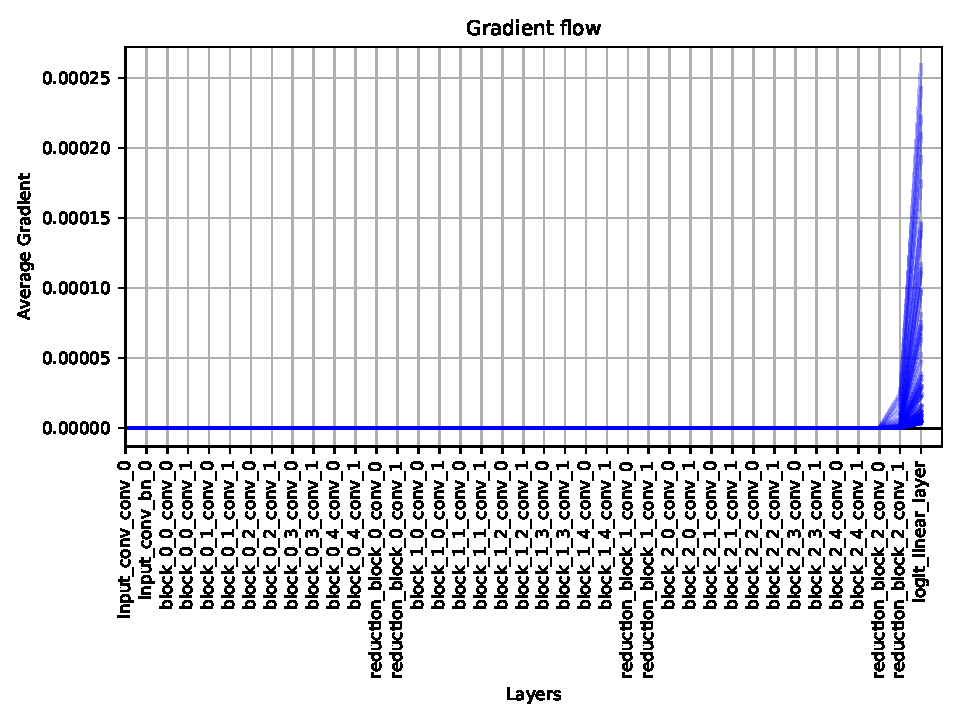
\includegraphics[width=\linewidth]{figures/vgg38-grad-flow.pdf}
    \caption{Gradient Flow for VGG38}
    \label{fig:grad_flow_38}
\end{figure}
}
}

%% Question Figure 4:
\newcommand{\questionFigureFour} {
\youranswer{Question Figure 4 - Replace this image with a figure depicting the training curves for the model with the best performance across experiments you have available. (Also edit the caption accordingly).
%
\begin{figure}
    \centering
    \begin{subfigure}[b]{\linewidth}
        \centering
        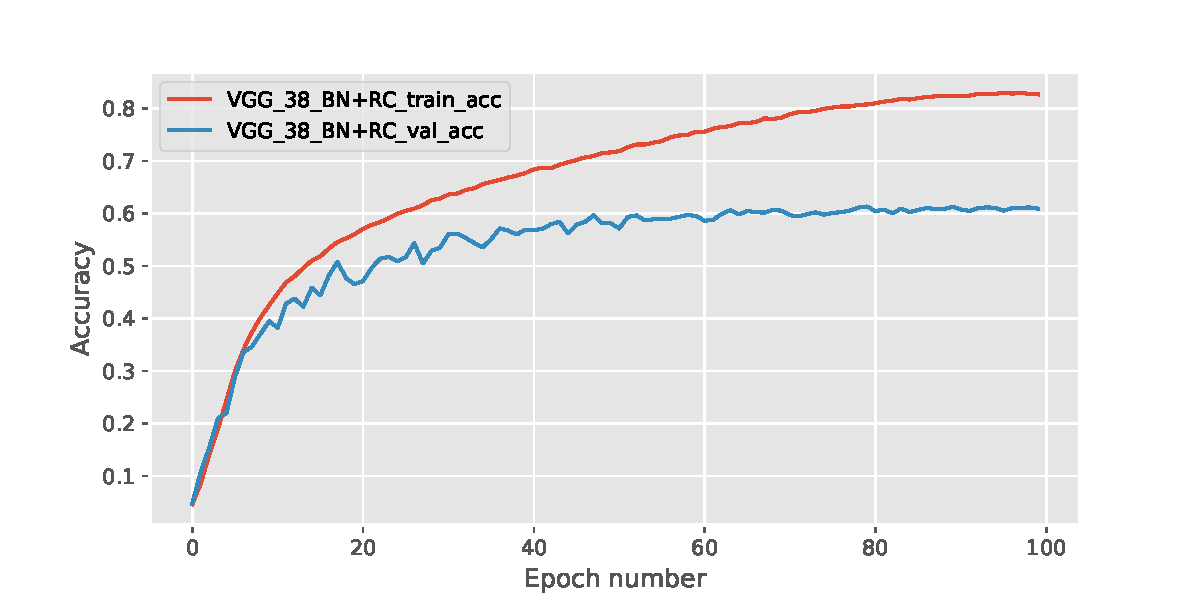
\includegraphics[width=\textwidth]{figures/best_model_accuracy_performance.pdf}
        \caption{Accuracy by epoch}
    \end{subfigure}
    %
    \begin{subfigure}[b]{\linewidth}
        \centering
        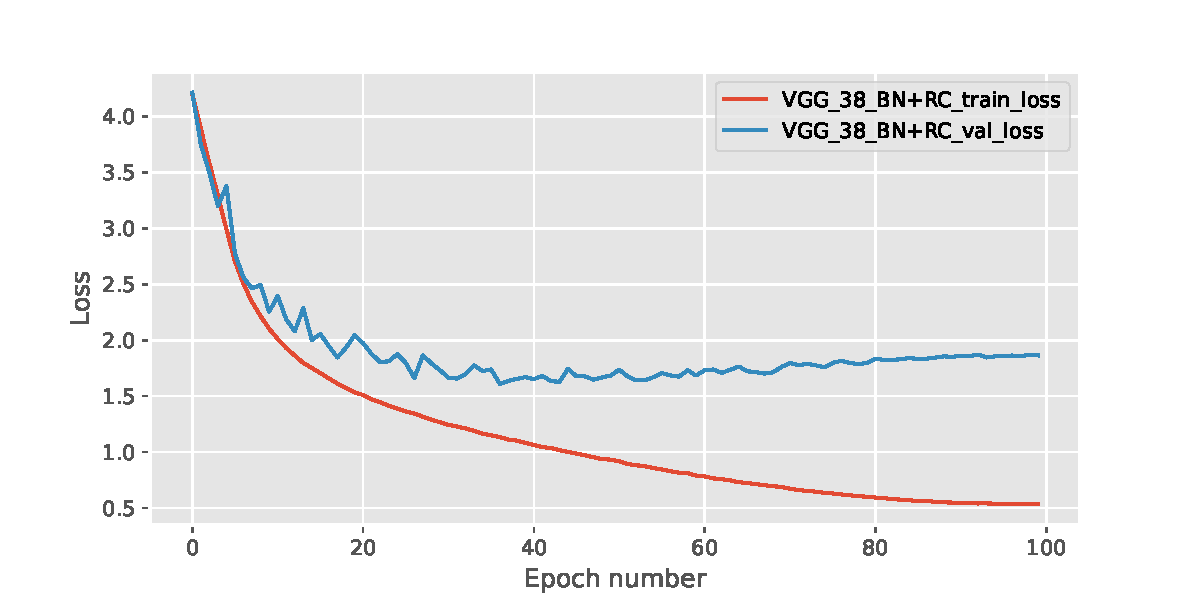
\includegraphics[width=\textwidth]{figures/best_model_loss_performance.pdf}
        \caption{Loss by epoch}
    \end{subfigure}
    \caption{Training and validation curves in terms of classification
accuracy (a) and loss (b) on the CIFAR100 dataset
for the best performing model: VGG38 BN+RC}
    \label{fig:grad_flow_bestModel}
\end{figure}
}
}

%% Question Figure 5:
\newcommand{\questionFigureFive} {
\youranswer{Question Figure 5 - Replace this image with a figure depicting the average gradient across layers, for the model with the best performance across experiments you have available. (Also edit the caption accordingly).
%
\begin{figure}[t]
    \centering
    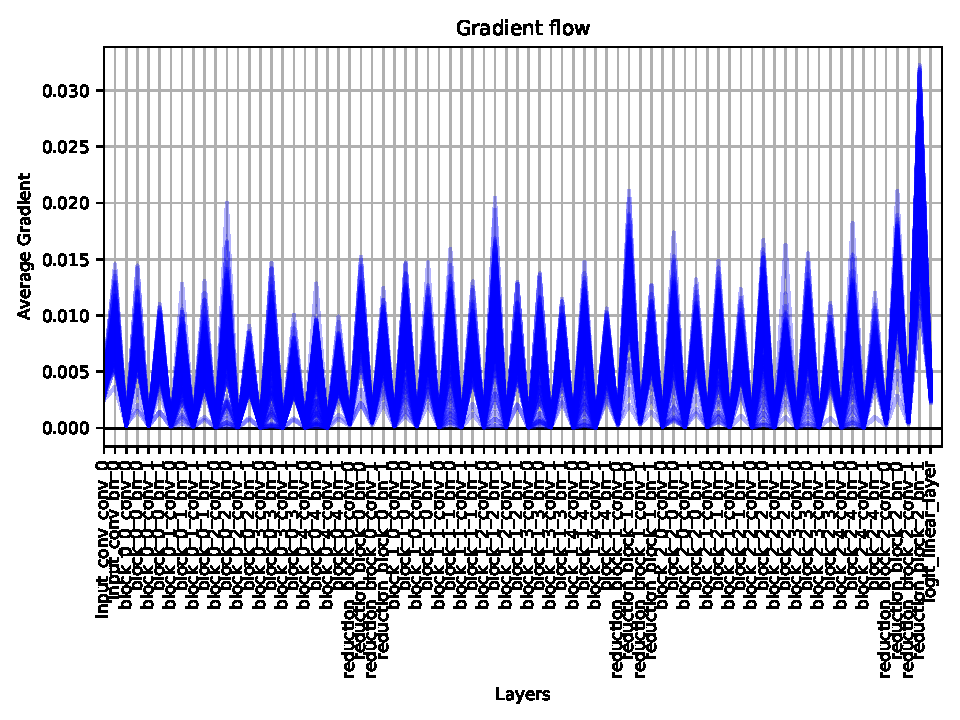
\includegraphics[width=\linewidth]{figures/best_model_gradient_flow.pdf}
    \caption{Gradient flow graphs for the best performing model: VGG38 BN+RC}
    \label{fig:grad_flow_bestModel}
\end{figure}
}
}

%% - - - - - - - - - - - - TABLES - - - - - - - - - - - - 

%% Question Table 1:
\newcommand{\questionTableOne} {
\youranswer{
Question Table 1 - Fill in Table 1 with the results from your experiments on 
\begin{enumerate}
    \item \textit{VGG38 BN (LR 1e-3)}, and 
    \item \textit{VGG38 BN + RC (LR 1e-2)}.
\end{enumerate}
%
\begin{table*}[t]
    \centering
    \begin{tabular}{lr|ccccc}
    \toprule
        Model                   & LR   & \# Params & Train loss & Train acc & Val loss & Val acc \\
    \midrule
        VGG08                   & 1e-3 & 60 K      &  1.74      & 51.59     & 1.95     & 46.84 \\
        VGG38                   & 1e-3 & 336 K     &  4.61      & 00.01     & 4.61     & 00.01 \\
        VGG38 BN                & 1e-3 &     339 K     &     1.47      &     57.57    &    1.98     &     47.52 \\
        VGG38 RC                & 1e-3 & 336 K     &  1.33      & 61.52     & 1.84     & 52.32 \\
        VGG38 BN + RC           & 1e-3 & 339 K     &  1.26      & 62.99     & 1.73     & 53.76 \\
        VGG38 BN                & 1e-2 & 339 K     &  1.70      & 52.28     & 1.99     & 46.72 \\
        VGG38 BN + RC           & 1e-2 &     339 K     &     0.57     &     82.02    &    1.79    &     61.8 \\
    \bottomrule
    \end{tabular}
    \caption{Experiment results (number of model parameters, Training and Validation loss and accuracy) for different combinations of VGG08, VGG38, Batch Normalisation (BN), and Residual Connections (RC), LR is learning rate.}
    \label{tab:CIFAR_results}
\end{table*} 
}
}

%% END of YOUR ANSWERS